\documentclass[11pt]{article}

% ---------------------------------------------------------------------------------------------------------------
% NovaQuantum: an SSA-based compiler on MLIR and LLVM, from a statically typed language to neutral-atom hardware.
% Self-contained: compiles with pdflatex (Overleaf, TeX Live, MiKTeX) using standard packages only.
% ---------------------------------------------------------------------------------------------------------------

\usepackage[margin=1in]{geometry}
\usepackage[T1]{fontenc}
\usepackage{lmodern}
\usepackage{microtype}
\usepackage{amsmath,amssymb}
\usepackage{booktabs}
\usepackage{graphicx}
\usepackage{xcolor}
\usepackage{listings}
\usepackage{tikz}
\usetikzlibrary{arrows.meta,positioning,shapes.geometric}
\usepackage[hidelinks]{hyperref}
\usepackage{caption}

\definecolor{codebg}{RGB}{246,247,250}
\definecolor{kw}{RGB}{40,70,160}
\definecolor{cm}{RGB}{110,110,110}
\lstdefinelanguage{Nova}{
  morekeywords={def,class,struct,extends,self,return,if,elif,else,while,do,for,switch,case,default,break,continue,
                pass,and,or,not,true,false,ignite,orbit,int,float,double,bool,string,Tensor,qubit,vector,map,none},
  sensitive=true, morecomment=[l]{\#}, morestring=[b]"
}
\lstdefinelanguage{MLIR}{
  morekeywords={func,scf,qnova,arith,return,yield,if,else},
  sensitive=true, morecomment=[l]{//}
}
\lstset{basicstyle=\ttfamily\small, backgroundcolor=\color{codebg}, keywordstyle=\color{kw}\bfseries,
        commentstyle=\color{cm}\itshape, frame=single, rulecolor=\color{black!15}, columns=fullflexible,
        keepspaces=true, showstringspaces=false, xleftmargin=4pt, xrightmargin=4pt, aboveskip=6pt, belowskip=6pt}

\title{\textbf{NovaQuantum: An SSA-Based Compiler on MLIR and LLVM\\
from a Statically Typed Language to Neutral-Atom Quantum Hardware}}
\author{Parhit Mathur\\
\small Source code: \url{https://github.com/parhitmtech/NovaQuantum}}
\date{November 2026}

\begin{document}
\maketitle

% ===============================================================================================================
\begin{abstract}
We present \emph{NovaQuantum}, a compiler built from scratch in C++ on MLIR and LLVM that compiles in two directions.
First, it compiles \emph{Nova}, a statically typed language with Python's syntax and built-in tensors, through a
custom MLIR dialect in static single-assignment (SSA) form and LLVM to native code, running programs up to
$215\times$ faster than Nova's reference interpreter while matching its output exactly on every program both
accept. Second, it compiles quantum circuits, written in Nova or imported from OpenQASM~3, for a neutral-atom
quantum computer. Circuits are represented in \texttt{qnova}, a dialect in which each qubit is an SSA value, so the
no-cloning theorem becomes a verifiable rule of the IR; they are decomposed into the machine's native gates
(Raman rotations and the Rydberg controlled-$Z$), optimized on SSA def-use chains, routed by \emph{physically moving
atoms} instead of inserting SWAP gates, scheduled into parallel layers under the Rydberg blockade constraint, and
lowered to a third dialect of timed hardware instructions. Every compiled circuit is checked on a statevector
simulator against the circuit as written. On benchmark circuits the optimizer removes 15--99\% of native gates; an
independent check against Qiskit agrees in all 88 comparisons; and a CUDA statevector simulator sustains 1.6\,TB/s
(77--81\% of peak memory bandwidth) on an NVIDIA A100, $256$--$529\times$ faster than one CPU core. Finally, we
describe the production tooling around the compiler: a diagnostics engine with stable error codes and error
recovery, a fuzzed front end, and a language server that gives editors the compiler's own errors in under a
millisecond per edit.
\end{abstract}

% ===============================================================================================================
\section{Introduction}

Machine-learning code is written in Python, a dynamically typed language whose performance comes from libraries
written in C++ and CUDA that the language itself cannot see into. Quantum software follows the same pattern: circuits
are built by Python libraries (Qiskit, Cirq, CUDA-Q) and handed to compilers as gate lists. In both cases the
program's structure, its types, and its invariants are invisible to the compiler that runs it.

This paper describes a compiler that takes the opposite approach. \emph{Nova} is a compiled, statically typed
language that reads like Python, with tensors, reverse-mode automatic differentiation, and qubits as first-class
types. Its compiler, \emph{NovaQuantum}, lowers programs through MLIR~\cite{mlir}, the multi-level intermediate
representation infrastructure behind many modern compilers, and LLVM~\cite{llvm}. Because the compiler sees the
whole program, it can type-check tensor code before it runs, enforce physical laws of quantum computing as rules of
its IR, and schedule circuits for a specific machine using the machine's own physics.

We target \emph{neutral-atom} quantum computers~\cite{saffman2010,bluvstein2022}, in which qubits are individual
atoms held in optical tweezers. Two properties of this hardware shape the compiler. Atoms can be physically moved,
so two qubits can be made adjacent without the SWAP gates that fixed-coupling hardware needs. And two-qubit gates are
performed by exciting atoms to Rydberg states, which forbids running two such gates close to each other at the same
time (the \emph{blockade} constraint), so the schedule must respect a geometric exclusion rule.

\paragraph{Contributions.}
\begin{enumerate}
  \item An SSA-based compiler for a statically typed, Python-syntax language, built on MLIR and LLVM: a hand-written
        front end, a custom \texttt{nova} dialect with declared memory effects, and dialect conversion to LLVM
        (Section~\ref{sec:classical}).
  \item \texttt{qnova}, a quantum dialect in which qubits are SSA values and a path-aware \texttt{LinearQubits}
        verifier enforces no-cloning, with decomposition, SSA-based optimization, routing by atom moves, and
        blockade-aware scheduling down to an \texttt{atom} dialect of timed hardware instructions
        (Section~\ref{sec:quantum}).
  \item A verification methodology that checks every compiled program against an independent reference:
        differential testing of native code against the interpreter, statevector simulation of every compiled
        circuit against the logical circuit, a cross-check against Qiskit through OpenQASM~3, and fuzzing of the
        front end (Section~\ref{sec:method}).
  \item A CUDA statevector simulator integrated as a compiler target, measured on an NVIDIA A100
        (Section~\ref{sec:results}).
  \item Production tooling: stable diagnostics with error recovery and a language server built on the compiler's
        own front end (Section~\ref{sec:tooling}).
\end{enumerate}

% ===============================================================================================================
\section{Background and Related Work}

\paragraph{SSA and MLIR.} Static single assignment form~\cite{cytron1991} gives every value exactly one definition,
which makes def-use chains explicit and turns many optimizations into local rewrites. MLIR~\cite{mlir} generalizes
SSA to extensible \emph{dialects} of operations with their own types, verifiers, and rewrite patterns, and lowers
programs progressively between them. Our design follows MLIR's multi-level approach: Nova programs and quantum
circuits each get a dialect at the level of abstraction where their invariants are easiest to state.

\paragraph{Quantum compilation.} Quantum compilers such as Qiskit's transpiler~\cite{qiskit} map logical circuits
onto hardware with limited connectivity, typically by inserting SWAP gates. OpenQASM~3~\cite{openqasm3} is the
common exchange format. Representing qubits as SSA values has been explored in quantum MLIR dialects and in
QIR-adjacent work; the key observation is that a \emph{linear} use discipline on qubit values encodes
no-cloning~\cite{wootters1982}.

\paragraph{Neutral-atom architectures.} Neutral-atom processors implement single-qubit gates with Raman lasers and
the two-qubit controlled-$Z$ through the Rydberg blockade~\cite{saffman2010}, and recent devices reconfigure qubit
connectivity by moving atoms with optical tweezers during a computation~\cite{bluvstein2022,bluvstein2024}. Atom
movement replaces SWAP-based routing but is slow compared to gates, which makes the cost model different from that
of superconducting hardware.

\paragraph{GPU kernels and statevector simulation.} Statevector simulation of $n$ qubits stores $2^n$ complex
amplitudes, and each gate touches all of them; it is therefore memory-bandwidth bound, which is the right metric for
a GPU simulator~\cite{cuquantum}. The project also includes hand-written CUDA and Triton~\cite{triton} matrix
multiplication kernels, summarized in Section~\ref{sec:results}.

% ===============================================================================================================
\section{System Overview}

Figure~\ref{fig:pipeline} shows the two compilation paths. Both share the front end; they diverge after the check
pass.

\begin{figure}[t]
\centering
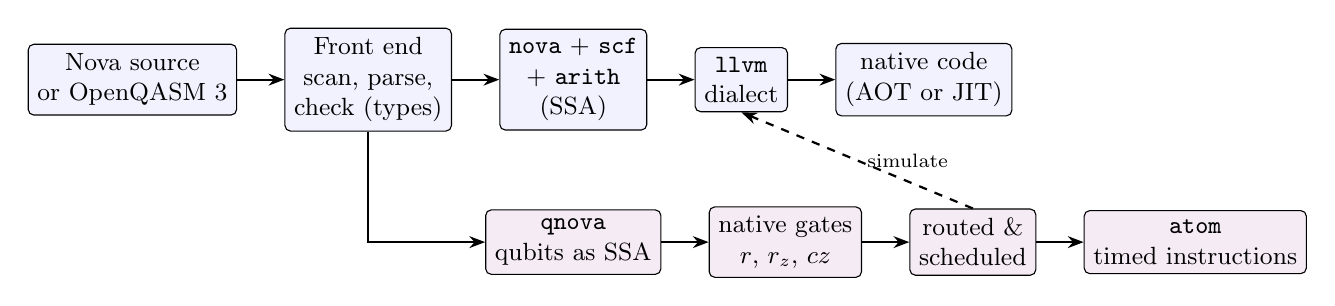
\begin{tikzpicture}[node distance=5mm and 6mm, every node/.style={font=\small},
  box/.style={draw, rounded corners=2pt, align=center, minimum height=8mm, fill=blue!5},
  q/.style={draw, rounded corners=2pt, align=center, minimum height=8mm, fill=violet!8},
  arr/.style={-{Stealth[length=2mm]}, thick}]
\node[box] (src) {Nova source\\or OpenQASM 3};
\node[box, right=of src] (fe) {Front end\\scan, parse,\\check (types)};
\node[box, right=of fe] (nova) {\texttt{nova} + \texttt{scf}\\+ \texttt{arith}\\(SSA)};
\node[box, right=of nova] (llvm) {\texttt{llvm}\\dialect};
\node[box, right=of llvm] (exe) {native code\\(AOT or JIT)};
\node[q, below=10mm of nova] (qn) {\texttt{qnova}\\qubits as SSA};
\node[q, right=of qn] (nat) {native gates\\$r$, $r_z$, $cz$};
\node[q, right=of nat] (sch) {routed \&\\scheduled};
\node[q, right=of sch] (atom) {\texttt{atom}\\timed instructions};
\draw[arr] (src) -- (fe); \draw[arr] (fe) -- (nova); \draw[arr] (nova) -- (llvm); \draw[arr] (llvm) -- (exe);
\draw[arr] (fe.south) |- (qn.west); \draw[arr] (qn) -- (nat); \draw[arr] (nat) -- (sch); \draw[arr] (sch) -- (atom);
\draw[arr, dashed] (sch.north) -- node[right, font=\scriptsize]{simulate} (llvm.south);
\end{tikzpicture}
\caption{The two compilation paths. Classical code lowers through the \texttt{nova} dialect to LLVM; quantum circuits
lower through \texttt{qnova} to hardware instructions, and are also compiled to native code that runs them on the
runtime's statevector simulator.}
\label{fig:pipeline}
\end{figure}

\begin{lstlisting}[language=Nova, caption={Quantum teleportation in Nova: qubits, gates from the built-in
\texttt{qpu} module, and classical feedback through \texttt{if}.}, label=lst:teleport]
ignite:
    qubit a = qpu.alloc()
    qubit b = qpu.alloc()
    qubit c = qpu.alloc()
    qpu.ry(a, 2.0943951023931953)    # the state to send: |1> with probability 0.75
    qpu.h(b)
    qpu.cx(b, c)                     # b and c entangled
    qpu.cx(a, b)
    qpu.h(a)
    bool m1 = qpu.measure(a)
    bool m2 = qpu.measure(b)
    if (m2):
        qpu.x(c)
    if (m1):
        qpu.z(c)
    qpu.probs(c)                     # |0>: 0.2500  |1>: 0.7500
\end{lstlisting}

% ===============================================================================================================
\section{Methodology}
\label{sec:method-design}

\subsection{Front end}
\label{sec:frontend}

The scanner turns Python-style indentation into \texttt{NEWLINE}, \texttt{INDENT} and \texttt{DEDENT} tokens, which
makes the language context-free over the token stream; we publish the complete grammar in EBNF. The parser is
recursive descent with precedence climbing and writes a \emph{flat parse tree in postorder}: each node holds only its
kind, its token, and the size of its subtree, so building the tree is one append per node and a node holds no
pointers. Names and types are resolved by a separate \emph{check pass} that produces, for each node, the entity it
names and its type. Functions with untyped parameters are generic and are compiled once per argument-type
combination (monomorphization), as C++ templates are.

\subsection{Classical path: SSA construction and lowering}
\label{sec:classical}

Lowering builds SSA directly from the checked tree. Each variable maps to the SSA value it currently holds; an
\texttt{if} produces results through \texttt{scf.if} (its results act as $\phi$-nodes); loop-carried variables become
block arguments of \texttt{scf.while}; and \texttt{break}, \texttt{continue} and early \texttt{return}, which
structured regions cannot express as jumps, become boolean flags.

The \texttt{nova} dialect is defined in TableGen (ODS). Tensor operations declare per-value memory effects
(\texttt{MemAlloc}, \texttt{MemRead}, \texttt{MemWrite}), and operations that can fail at run time declare an effect
on a dedicated \texttt{runtime\_error} resource. This lets MLIR's generic passes (common-subexpression elimination,
loop-invariant code motion, canonicalization) optimize tensor code without reordering or deleting an operation whose
error the program could observe. Integer division by zero, undefined behavior in LLVM, is an explicit check
operation that canonicalization removes when the divisor is a non-zero constant. Dialect conversion with a type
converter then maps tensors to pointers and each operation to a call into a C runtime, and MLIR's standard
conversions produce the \texttt{llvm} dialect. The result is compiled ahead of time to an executable, or compiled in
memory with LLVM's ORC JIT and run, which lets a sandboxed cloud IDE run programs without writing an executable.

\subsection{Quantum path: the \texttt{qnova} dialect}
\label{sec:quantum}

\paragraph{Qubits as SSA values.} In \texttt{qnova} every gate consumes its qubit values and produces new ones. A
Nova variable that holds a qubit is rebound to the new value after each gate, using the same SSA construction as
for ordinary variables; a qubit flowing through an \texttt{if} becomes the \texttt{if}'s result:

\begin{lstlisting}[language=MLIR]
%bit, %a1 = qnova.measure %a0
%c1 = scf.if %bit -> (!qnova.qubit) {   // the corrected qubit: a phi of the circuit's wire
  %x = qnova.x %c0
  scf.yield %x : !qnova.qubit
} else {
  scf.yield %c0 : !qnova.qubit
}
\end{lstlisting}

\paragraph{No-cloning as an IR invariant.} A quantum state cannot be copied~\cite{wootters1982}. We enforce this
twice. The check pass rejects Nova code that would copy a state (assigning a qubit, passing one to a function, or
giving one gate the same qubit twice). In the IR, a \texttt{LinearQubits} trait verifies that each qubit value is
consumed at most once on every control-flow path, treating the two branches of an \texttt{if} as separate paths.
Any transformation that duplicated a qubit would therefore fail verification immediately.

\paragraph{Decomposition into native gates.} The \texttt{--qnova-decompose} pass rewrites logical gates
($H$, $X$, $CX$, $CP(\theta)$, SWAP, \dots) into the machine's native set: Raman rotations $r(\theta,\phi)$, phase
rotations $r_z(\theta)$, and the Rydberg controlled-$Z$.

\paragraph{Optimization on def-use chains.} Because qubits are SSA values, the gate that last acted on a qubit is its
value's defining operation, so peephole rules are local pattern matches: self-inverse gates cancel, consecutive
rotations merge, and diagonal gates commute through $cz$. Gates whose effect cannot be observed are removed: diagonal
gates on freshly allocated qubits or immediately before measurement, and gates on qubits that are never measured,
which is justified by the no-signaling theorem.

\paragraph{Routing by atom moves.} Qubits are placed on a grid of trap sites (a checkerboard placement). When a
$cz$ needs two atoms within interaction range, the router \emph{moves an atom} with an optical tweezer rather than
inserting SWAP gates, and records the move as an operation with its distance.

\paragraph{Scheduling under the blockade.} Operations are packed into parallel layers of three kinds: Raman
(single-qubit), Rydberg (two-qubit), and move. Two $cz$ gates may share a Rydberg layer only if their atoms are
farther apart than the blockade radius. Each trap site is a resource, so the scheduler also orders operations that
would place two atoms on the same site; this dependence was added after simulation exposed a collision bug that was
invisible at the gate level (Section~\ref{sec:results}).

\paragraph{Timed hardware instructions.} A third dialect, \texttt{atom}, is the machine's instruction stream: atom
loads, Raman pulses and phase shifts on sites, tweezer moves, and one \emph{global} Rydberg pulse per layer, each
with a start time and duration under a configurable timing model.

\paragraph{Simulation and interoperability.} The runtime includes a statevector simulator, parallelized with OpenMP
on the CPU and implemented with one coalesced CUDA kernel per gate on the GPU. OpenQASM~3 is imported to and
exported from \texttt{qnova} by \texttt{nova-translate}, so circuits from Qiskit or CUDA-Q enter the same pipeline.

% ===============================================================================================================
\section{Experimental Procedure}
\label{sec:method}

We evaluate correctness first and performance second; every result in Section~\ref{sec:results} is produced by a
script in the repository and, except for the GPU measurements, by continuous integration on every change.

\paragraph{Differential testing (classical path).} Every program in the language's test suite and benchmark set is
compiled to a native executable and also run by Nova's reference interpreter. Their standard output, standard
error, and exit status must match. A runtime error matches when both report the same line, error code and message.

\paragraph{Simulation of every compiled circuit (quantum path).} For each benchmark circuit, the probabilities of the
compiled native circuit, and of the timed hardware program executed site by site, must equal those of the logical
circuit as written.

\paragraph{Independent cross-check.} Circuits are exported to OpenQASM~3 and simulated by Qiskit~2.6.2, an
implementation independent of ours; conversely, Qiskit's random circuits are imported and run as written, as
native gates, and as hardware instructions.

\paragraph{Benchmarks.} Classical: naive recursive Fibonacci (call-heavy), an integer loop, and a vector sum,
compared with the interpreter and with equivalent C compiled by \texttt{clang -O2}. Quantum: GHZ state preparation,
a quantum Fourier transform followed by its inverse, and random circuits of 120 and 300 gates.

\paragraph{GPU simulator.} Measured on an NVIDIA A100-80GB on Arizona State University's SOL cluster, against the
OpenMP CPU simulator on 1 and 16 cores, after a warm-up run (an early measurement without it was distorted by
OpenMP thread start-up). We report effective memory bandwidth, the bound that matters for statevector simulation.

\paragraph{Robustness.} The front end (scanner, parser, check pass) is fuzzed with libFuzzer under AddressSanitizer
and UndefinedBehaviorSanitizer, seeded with the test programs and the standard library; CI fuzzes it on every
change.

% ===============================================================================================================
\section{Results}
\label{sec:results}

\subsection{Classical path}

Table~\ref{tab:classical} compares compiled code with the reference interpreter. Call-heavy and loop-heavy code
speeds up by two orders of magnitude and lands within a small factor of C, because MLIR and LLVM see ordinary SSA
integer code. Recursion that does little work per call (\texttt{fibonacci}) gains least: the interpreter already
memoizes pure recursive functions automatically, which the native path does not yet do.

\begin{table}[h]
\centering
\caption{Native code compiled through MLIR and LLVM against Nova's interpreter, and against equivalent C.}
\label{tab:classical}
\begin{tabular}{lrrrr}
\toprule
Benchmark & Interpreter & Nova native & Speed-up & C, \texttt{clang -O2} \\
\midrule
\texttt{calls} (naive $\mathit{fib}(30)$, 1.3M calls) & 633 ms & 2.9 ms & \textbf{215$\times$} & 2.5 ms \\
\texttt{int\_loop} (3M iterations)                     & 159 ms & 1.0 ms & \textbf{157$\times$} & 2.1 ms \\
\texttt{fibonacci} ($\mathit{fib}(35)$)                &  53 ms &  26 ms & 2.1$\times$         &  34 ms \\
\bottomrule
\end{tabular}
\end{table}

Differential testing compiles 30 programs natively, and \textbf{all 30 behave exactly as the interpreter does}. It
found two real bugs during development: the interpreter printed a tensor's handle instead of its elements, and
integer division by zero was undefined behavior in the generated LLVM IR; both are fixed.

\subsection{Quantum path}

Table~\ref{tab:quantum} reports circuits compiled for the neutral-atom machine. ``Saved'' is the fraction of native
gates the optimizer removes. The quantum Fourier transform followed by its inverse is the identity, and the
optimizer reduces it to 4 gates from 764 (99\%) through repeated inverse cancellation and rotation merging; random
circuits, which have little structure to exploit, still lose 15--27\% of their gates. All compiled circuits, and their
hardware programs, give the same probabilities as the logical circuits.

\begin{table}[h]
\centering
\caption{Benchmark circuits compiled for the neutral-atom machine. Gate and move times are those of the timed
hardware program, without the final readout.}
\label{tab:quantum}
\begin{tabular}{lrrrrrrrr}
\toprule
Circuit & Qubits & Native & Compiled & Saved & Moves & Layers & Gate time & Move time \\
\midrule
GHZ                     & 12 &   57 &  45 & 21\%          &  7 &  26 &  10.9\,$\mu$s &   80.0\,$\mu$s \\
QFT, then its inverse   &  8 &  764 &   4 & \textbf{99\%} &  0 &   1 &   1.0\,$\mu$s &    0 \\
random, 120 gates       &  8 &  483 & 355 & \textbf{27\%} & 26 & 244 & 109.5\,$\mu$s &  725.2\,$\mu$s \\
random, 300 gates       & 12 & 1026 & 867 & 15\%          & 72 & 496 & 219.3\,$\mu$s & 1727.4\,$\mu$s \\
\bottomrule
\end{tabular}
\end{table}

\paragraph{Movement dominates run time.} Moves take 3--8$\times$ as long as all the gates combined, so on this
machine model routing, not gate count, determines execution time. This motivates move-aware placement as the next
optimization target.

\paragraph{A bug only the hardware program revealed.} Executing the timed hardware program site by site on the
simulator exposed a scheduler bug in which two atoms were moved onto the same trap site in one layer. The logical
and native circuits were correct, so gate-level checks could not see it. Treating each site as a scheduling resource
fixed it, and the site-level simulation is now part of every CI run.

\paragraph{Agreement with Qiskit.} Qiskit's independent simulator agrees with NovaQuantum in \textbf{all 88
comparisons}: NovaQuantum's circuits exported as written and as compiled, and Qiskit's random circuits imported and
run as written, as native gates, and as hardware instructions.

\subsection{GPU statevector simulator}

On the A100-80GB the GPU simulator matches the CPU simulator to $10^{-17}$ and sustains \textbf{1.6\,TB/s, 77--81\%
of the GPU's peak memory bandwidth}. At 20--24 qubits it is \textbf{$256$--$529\times$ faster than one CPU core} and
$21$--$37\times$ faster than 16 cores; a 28-qubit circuit of 695 gates runs in 3.1\,s. Since every gate reads and
writes the whole statevector, running near peak bandwidth is close to the best this algorithm can do.

\subsection{GPU kernels}

As part of the same project, matrix multiplication was written by hand in CUDA in four steps (naive, tiled, register
blocked, and pipelined with \texttt{cp.async} double buffering) and in Triton. On a $4096^3$ product the pipelined
CUDA kernel reaches 82\% of cuBLAS; Triton reaches 95\% in FP32, and up to 100\% of cuBLAS with tensor cores
(TF32) depending on the shape, with 111\,TFLOP/s at $4096^3$.

\subsection{Robustness of the front end}

In a 10-minute run, the fuzzer executed 387{,}899 inputs with no crash, hang, or sanitizer report. An earlier run
found a crash in released code (a class defined twice made the check pass read past an array); it is fixed and kept
as a regression input.

% ===============================================================================================================
\section{Production Tooling}
\label{sec:tooling}

A compiler is used through its error messages. Every error and warning goes through one diagnostics engine as a
stable code, a source range, a message, notes and machine-applicable fixes, printed in the
\texttt{file:line:col:} form editors read, or as JSON for tools. After a syntax error the parser replaces the failed
statement with an error node and resynchronizes at the next one, built on its existing failure mode without C++
exceptions; only the first syntax error of a line is reported, so one run reports every mistake without cascades.
Runtime errors point at the failing expression with the call stack, at a measured cost within the noise of the
interpreter benchmarks.

\texttt{nova-lsp}, a Language Server Protocol implementation, is linked with the same front end, so the editor
shows exactly the compiler's errors; a full re-analysis per edit takes under a millisecond on the example programs.
It provides hover, go to definition, completion (including member completion while the line does not yet parse),
signature help and quick fixes, and backs a VS Code extension tested in a real editor in continuous integration.

% ===============================================================================================================
\section{Discussion and Limitations}

The native path does not yet cover all of Nova: 99 test programs use features (strings, containers, some class
forms) that lowering reports as not supported, and imports (\texttt{orbit}) are handled only by the interpreter.
Quantum circuits with classical feedback compile to native gates but are not yet scheduled into hardware
instructions. The timing model is configurable but not calibrated against a specific device, so absolute times
illustrate trade-offs rather than predict hardware runs. Finally, the type checker reports names and types only
once a file parses; while a line is being typed, the language server answers from the last version that did.

% ===============================================================================================================
\section{Conclusion}

NovaQuantum shows that one SSA-based compiler stack on MLIR and LLVM can serve both a Python-syntax, statically typed
language for machine learning and quantum circuits for neutral-atom hardware. Representing qubits as SSA values
makes no-cloning a verifiable invariant and turns circuit optimization into local rewrites on def-use chains;
routing by atom movement and blockade-aware scheduling capture the physics of the target machine; and systematic
checking against independent references (the interpreter, the logical circuit, Qiskit, and a fuzzer) caught real
bugs that gate-level testing could not. Future work includes move-aware placement, scheduling of circuits with
classical feedback, calibrated timing models, and wider native coverage of the language.

% ===============================================================================================================
\begin{thebibliography}{99}

\bibitem{mlir} C.~Lattner, M.~Amini, U.~Bondhugula, A.~Cohen, A.~Davis, J.~Pienaar, R.~Riddle, T.~Shpeisman,
N.~Vasilache, and O.~Zinenko. MLIR: Scaling compiler infrastructure for domain specific computation. In
\emph{Proc.\ IEEE/ACM International Symposium on Code Generation and Optimization (CGO)}, 2021.

\bibitem{llvm} C.~Lattner and V.~Adve. LLVM: A compilation framework for lifelong program analysis and
transformation. In \emph{Proc.\ CGO}, 2004.

\bibitem{cytron1991} R.~Cytron, J.~Ferrante, B.~K.~Rosen, M.~N.~Wegman, and F.~K.~Zadeck. Efficiently computing
static single assignment form and the control dependence graph. \emph{ACM Transactions on Programming Languages and
Systems}, 13(4):451--490, 1991.

\bibitem{wootters1982} W.~K.~Wootters and W.~H.~Zurek. A single quantum cannot be cloned. \emph{Nature},
299:802--803, 1982.

\bibitem{saffman2010} M.~Saffman, T.~G.~Walker, and K.~M{\o}lmer. Quantum information with Rydberg atoms.
\emph{Reviews of Modern Physics}, 82(3):2313--2363, 2010.

\bibitem{bluvstein2022} D.~Bluvstein et al. A quantum processor based on coherent transport of entangled atom
arrays. \emph{Nature}, 604:451--456, 2022.

\bibitem{bluvstein2024} D.~Bluvstein et al. Logical quantum processor based on reconfigurable atom arrays.
\emph{Nature}, 626:58--65, 2024.

\bibitem{openqasm3} A.~Cross et al. OpenQASM 3: A broader and deeper quantum assembly language. \emph{ACM
Transactions on Quantum Computing}, 3(3), 2022.

\bibitem{qiskit} A.~Javadi-Abhari et al. Quantum computing with Qiskit. arXiv:2405.08810, 2024.

\bibitem{triton} P.~Tillet, H.~T.~Kung, and D.~Cox. Triton: An intermediate language and compiler for tiled neural
network computations. In \emph{Proc.\ ACM SIGPLAN International Workshop on Machine Learning and Programming
Languages (MAPL)}, 2019.

\bibitem{cuquantum} H.~Bayraktar et al. cuQuantum SDK: A high-performance library for accelerating quantum science.
In \emph{Proc.\ IEEE International Conference on Quantum Computing and Engineering (QCE)}, 2023.

\end{thebibliography}

\end{document}
